\chapter{Results}
\label{cha:results}
This chapter details the results of the project, along with views of the user interface and the final findings of the system.

\section{Feature Extraction}
The analysis of results is a semi-automated process carried out by checking which tweets were said to contain software and which did not. In total, 3268 tweets were retrieved from Twitter and stored in the MySQL database. These have all been through the feature extraction process, and 1168 of these are said to mention software or operating systems, leaving 2100 that do not. Of these tweets, roughly 10\%, i.e. 350, were manually tagged purely with software names. Comparing these results produces the accuracy measures shown in Tables~\ref{tbl:truefalse} and \ref{tbl:measures}.

\begin{table}[h]
\begin{center}
\begin{tabular}{|c|c|c|c|c|}\hline
True Positives&True Negatives&False Positives&False Negatives&\textbf{Total}\\\hline
117&162&32&56&\textbf{367}\\\hline
\end{tabular}
\end{center}
\caption{Results from comparing manual and automated tagging}
\label{tbl:truefalse}
\end{table}

\begin{table}[h]
\begin{center}
\begin{tabular}{|c|c|c|c|}\hline
Precision&Recall&Specificity&\textbf{F-measure}\\\hline
0.79&0.68&0.84&\textbf{0.73}\\\hline
\end{tabular}
\end{center}
\caption{Precision, recall, specificity and F-measure}
\label{tbl:measures}
\end{table}

\section{GUI}
The GUI for this system has been implemented to the design requirements stated in Section~\ref{sec:guid}. All pages display a navigation bar allowing access to the Tweet Retrieval subsystem as well as the analysis pages. The home page displays the top ten tweeted software as found by the application. This can be seen in Figure~\ref{fig:gui1}. The elements in this list are clickable hyperlinks to their respective analysis pages.

\begin{figure}[h]
\begin{center}
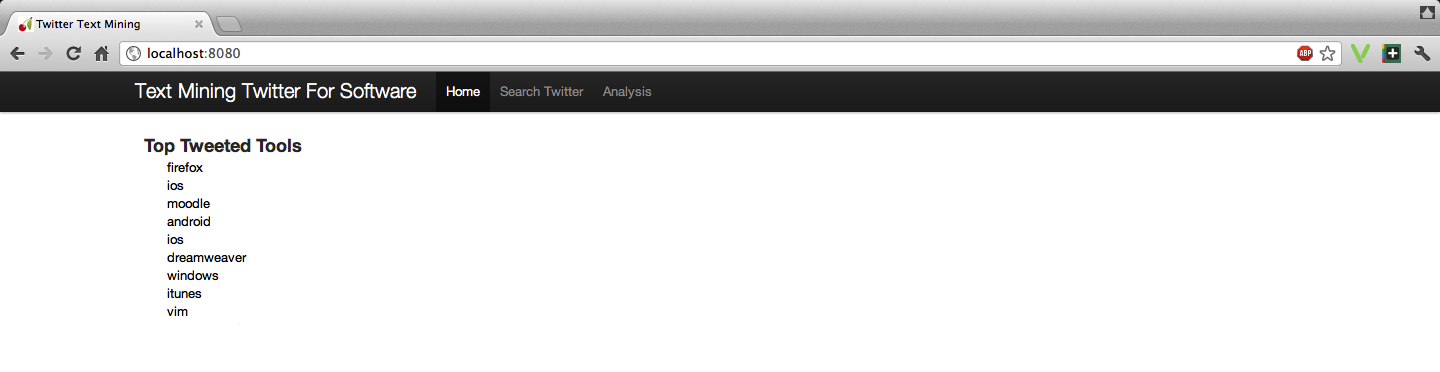
\includegraphics[width=15cm]{gui1}
\end{center}
\caption{The web application's home page}
\label{fig:gui1}
\end{figure}

The search page asks users to enter a single query term as shown in Figure~\ref{fig:gui2}. This should ideally be the name of some software, operating system or programming language. After completing this search, the page displayed in Figure~\ref{fig:gui3} shows all retrieved tweets corresponding to the given query term, after being sent through the feature extraction process.

\begin{figure}[h]
\begin{center}
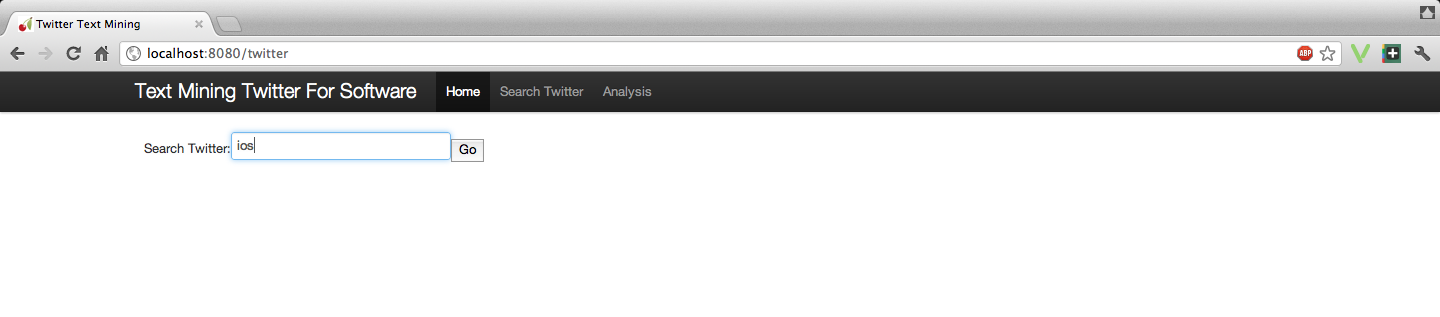
\includegraphics[width=15cm]{gui2}
\end{center}
\caption{The web application's search page}
\label{fig:gui2}
\end{figure}

\begin{figure}[h]
\begin{center}
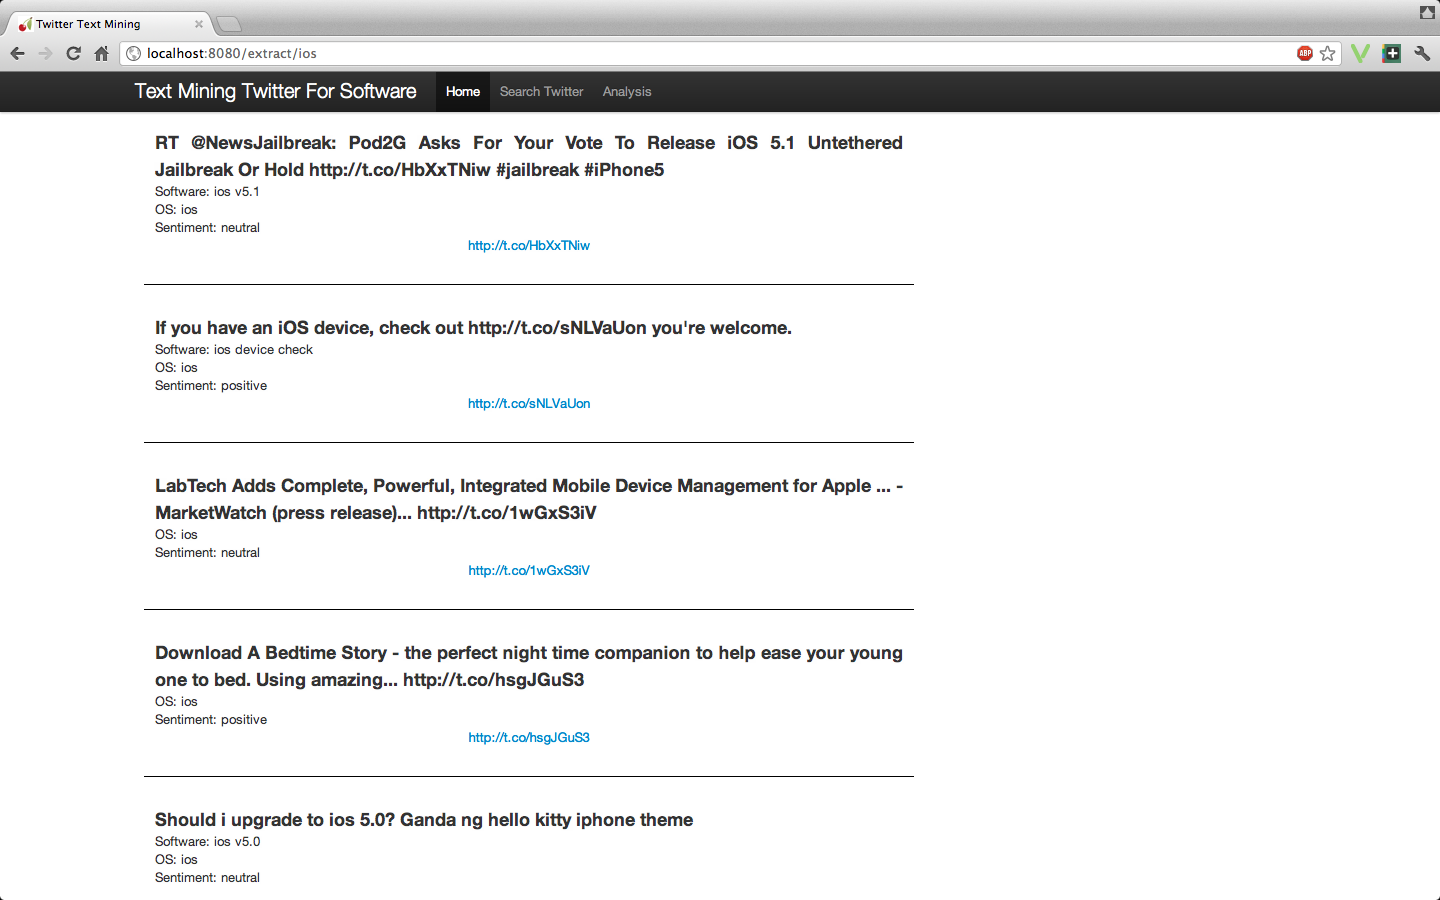
\includegraphics[width=15cm]{gui3}
\end{center}
\caption{The web application's extracted features page}
\label{fig:gui3}
\end{figure}

The final requirement is to show display the key information to the user. This involves displaying a pie chart representing the sentiment of tweets mentioning the selected software, and is shown in Figures~\ref{fig:gui4} and \ref{fig:gui5}.

\begin{figure}[h]
\begin{center}
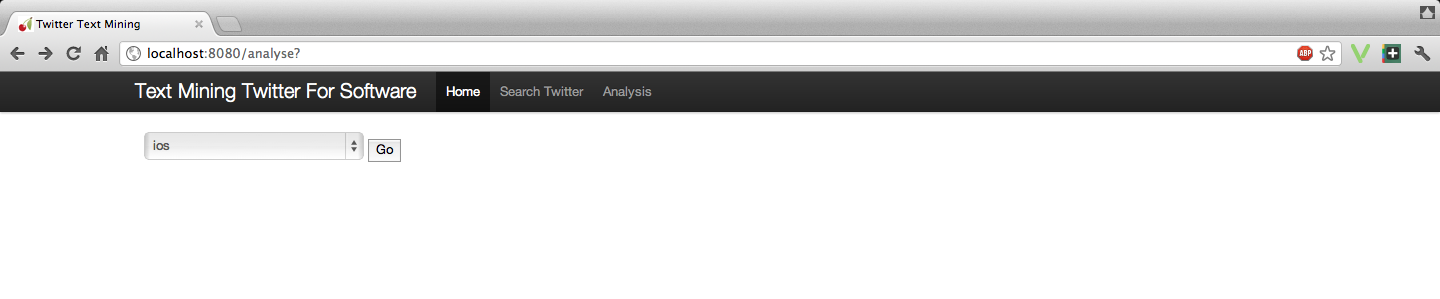
\includegraphics[width=15cm]{gui4}
\end{center}
\caption{The web application's analysis dropdown menu}
\label{fig:gui4}
\end{figure}

\begin{figure}[h]
\begin{center}
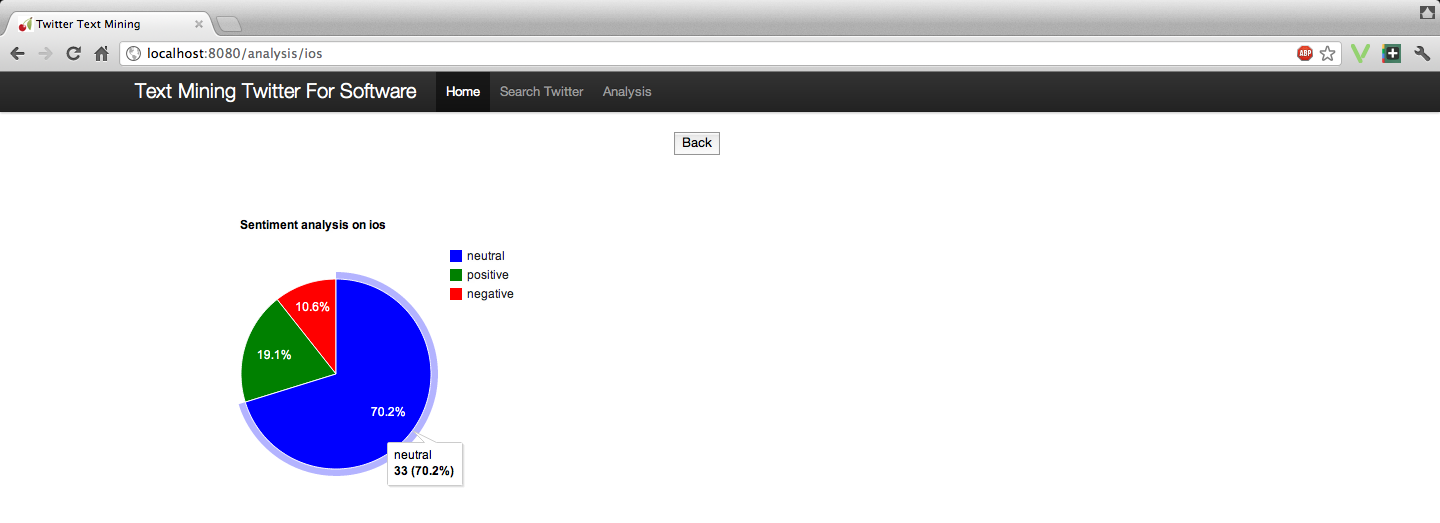
\includegraphics[width=15cm]{gui5}
\end{center}
\caption{The web application's analysis page for a specified piece of software}
\label{fig:gui5}
\end{figure}
